\iffalse
\let\negmedspace\undefined
\let\negthickspace\undefined
\documentclass[journal,12pt,onecolumn]{IEEEtran}
\usepackage{cite}
\usepackage{amsmath,amssymb,amsfonts,amsthm}

\usepackage{graphicx}
\usepackage{textcomp}
\usepackage{xcolor}
\usepackage{txfonts}
\usepackage{listings}
\usepackage{enumitem}
\usepackage{mathtools}
\usepackage{gensymb}
\usepackage[breaklinks=true]{hyperref}
\usepackage{tkz-euclide} % loads  TikZ and tkz-base
\usepackage{listings}
\usepackage{gvv}
\usepackage{booktabs}

%
%\usepackage{setspace}
%\usepackage{gensymb}
%\doublespacing
%\singlespacing

%\usepackage{graphicx}
%\usepackage{amssymb}
%\usepackage{relsize}
%\usepackage[cmex10]{amsmath}
%\usepackage{amsthm}
%\interdisplaylinepenalty=2500
%\savesymbol{iint}
%\usepackage{txfonts}
%\restoresymbol{TXF}{iint}
%\usepackage{wasysym}
%\usepackage{amsthm}
%\usepackage{iithtlc}
%\usepackage{mathrsfs}
%\usepackage{txfonts}
%\usepackage{stfloats}
%\usepackage{bm}
%\usepackage{cite}
%\usepackage{cases}
%\usepackage{subfig}
%\usepackage{xtab}
%\usepackage{longtable}
%\usepackage{multirow}

%\usepackage{algpseudocode}
%\usepackage{enumitem}
%\usepackage{mathtools}
%\usepackage{tikz}
%\usepackage{circuitikz}
%\usepackage{verbatim}
%\usepackage{tfrupee}
%\usepackage{stmaryrd}
%\usetkzobj{all}
%    \usepackage{color}                                            %%
%    \usepackage{array}                                            %%
%    \usepackage{longtable}                                        %%
%    \usepackage{calc}                                             %%
%    \usepackage{multirow}                                         %%
%    \usepackage{hhline}                                           %%
%    \usepackage{ifthen}                                           %%
  %optionally (for landscape tables embedded in another document): %%
%    \usepackage{lscape}     
%\usepackage{multicol}
%\usepackage{chngcntr}
%\usepackage{enumerate}

%\usepackage{wasysym}
%\documentclass[conference]{IEEEtran}
%\IEEEoverridecommandlockouts
% The preceding line is only needed to identify funding in the first footnote. If that is unneeded, please comment it out.

\newtheorem{theorem}{Theorem}[section]
\newtheorem{problem}{Problem}
\newtheorem{proposition}{Proposition}[section]
\newtheorem{lemma}{Lemma}[section]
\newtheorem{corollary}[theorem]{Corollary}
\newtheorem{example}{Example}[section]
\newtheorem{definition}[problem]{Definition}
%\newtheorem{thm}{Theorem}[section] 
%\newtheorem{defn}[thm]{Definition}
%\newtheorem{algorithm}{Algorithm}[section]
%\newtheorem{cor}{Corollary}
\newcommand{\BEQA}{\begin{eqnarray}}
\newcommand{\EEQA}{\end{eqnarray}}
\newcommand{\define}{\stackrel{\triangle}{=}}
\theoremstyle{remark}
\newtheorem{rem}{Remark}

%\bibliographystyle{ieeetr}
\begin{document}
%

\bibliographystyle{IEEEtran}


\vspace{3cm}

\title{
%	\logo{
Gate 2021 Assignment 

\large{EE:1205 Signals and Systems}

Indian Institute of Technology, Hyderabad
%	}
}
\author{Abhey Garg

EE23BTECH11202
}	


% make the title area
\maketitle



%\tableofcontents


\renewcommand{\thefigure}{\theenumi}
\renewcommand{\thetable}{\theenumi}
%\renewcommand{\theequation}{\theenumi}

\section{Question IN 02}
Consider a unity feedback configuration with a plant and a PID controller as shown in the figure. $G(s) = \frac{1}{(s+1)(s+3)} $ and $ C(s) = \frac{K(s+3+j)(s+3-j)}{s}$ with K being scalar . The closed loop is :
\begin{center}
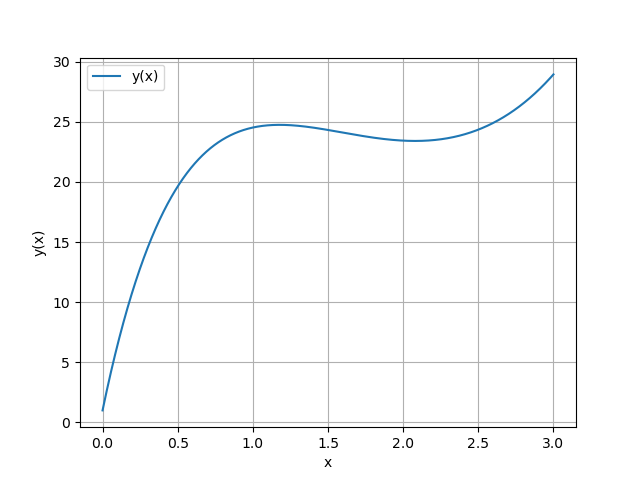
\includegraphics[width=0.5\textwidth]{2021/IN/29/figs/figure1.jpg}
\end{center}
\begin{enumerate}
\item[A]only stable for $K < 0$
\item[B]stable for all value of K
\item[C]only stable for $K > 0$
\item[D]only stable for K between –1 and +1
\end{enumerate}
\section{Solution}
\fi
\begin{table}[ht]
\centering
\setlength{\extrarowheight}{8pt}
\caption{Input Parameters}
\begin{tabular}{|c|l|l|} 
\hline
\textbf{Parameter} & \textbf{Used to denote} & \textbf{Values} \\
\hline
$n$ & Number of forward paths & \multicolumn{1}{|p{1.3cm}|}{\centering $1$ }\\
\hline
$\Delta_k$ & The value of $\Delta$ which is not touching the $k^{th} $ forward path & \multicolumn{1}{|p{1.3cm}|}{\centering $\Delta = 1 $ } \\
\hline
$\Delta$ & 1 - sum of the loop gains & \multicolumn{1}{|p{1.3cm}|}{\centering $1-G(s)C(s)$ } \\
\hline
$P$ & $k^{th}$ forward path gain & \multicolumn{1}{|p{1.3cm}|}{\centering $P = G(s)C(s)$ } \\
\hline
\end{tabular}
 \vspace{4mm}
 \label{tab:table0}
\end{table}
According to Mason's gain formula , transfer function can be given as :
\begin{align}
\text{TF } &= \frac{\sum_{k-1}^{n} P_k \Delta_k}{\Delta} = \frac{P\Delta_1}{\Delta} \\
&= \frac{G(s)C(s) }{1 + G(s)C(s)}
\end{align}
Substituting values of G(s) and C(s) : 
\begin{align}
\text{TF} &= \frac{k(s+3+j)(s+3-j)}{(s+1)(s+3) + k(s+3+j)(s+3-j)}
\end{align}
For the system to be stable , the real part of the pole should be negative.\\
\begin{align}
s(s+1)(s+3) + K((s+3)^2 - j^2) = 0\\
s^3 + s^2(K+4) +s(3+6K) +10  = 0
\end{align}
For stability we need :
\begin{align}
(K+4)(3+6K) > 10\\
\text{from Routh Hurwitz Criterion}\\
[ \because as^3 + bs^2 + cs + d = 0\text{ for stability } bc>ad]\\
3K +6K^2 +12 +24K > 10\\
6K^2 +24K +2 >0 
\end{align}
\begin{center}
\includegraphics[width=0.5\textwidth]{2021/IN/29/figs/figure2.png}
\end{center}
If k =1 then above equation is valid, hence option A is wrong.\\
If k = –1 then above equation is invalid, hence option B is wrong.\\
If k = 2 then also above equation is valid, hence option D is wrong.\\
If $k > 0$ then always above equation is valid, hence option C is correct.

%\end{document}
